\documentclass[11pt]{article}
\usepackage[a4paper,margin=25mm]{geometry}
\usepackage[T1]{fontenc}
\usepackage{lmodern}
\usepackage{amsmath,amssymb,amsthm,booktabs,microtype}
\usepackage{tikz}
\usepackage[colorlinks=true,linkcolor=blue,urlcolor=blue,citecolor=blue]{hyperref}
\numberwithin{equation}{section}
\newtheorem{theorem}{Theorem}[section]
\newtheorem{lemma}[theorem]{Lemma}
\newtheorem{corollary}[theorem]{Corollary}
\newcommand{\cost}{\operatorname{cost}}
\newcommand{\OPT}{\operatorname{OPT}}
\newcommand{\MS}{\mathrm{MS}}
\newcommand{\dep}{\operatorname{depth}}
\newcommand{\polylog}{\operatorname{polylog}}
\newcommand{\lgit}[1]{\log^{(#1)}}
\setlength{\emergencystretch}{3em}
\hypersetup{pdftitle={A smaller competitive ratio for standard multi-splay},
pdfauthor={Research note, 2 October 2026}}
\title{A smaller competitive ratio for standard multi-splay\\
\large A comparison with the Tango-squared construction}
\author{Research note}
\date{2 October 2026}
\begin{document}
\maketitle
\begin{abstract}
We explain a hand derivation, from the current Splay and Tango-squared
proofs, of the bound
\[
 \cost_{\MS}(X)=O\!\left((\OPT(X)+n)
 (1+\lgit{3}n)^2(1+\lgit{4}n)^2\right)
\]
for the unchanged standard multi-splay algorithm. The proof represents
its exact switches as one persistent word of splits and joins, extends
the Splay comparison accounting to this common forest, and constructs
a compatible comparator using the Tango-squared representation.
We include the endpoint and switch-order reductions needed for ordinary
node queries. The proof uses the existing Tango-squared lower bound
and physical unfolding lemmas. The new composition is a hand proof,
not a newly Lean-verified theorem. It does not establish the stronger
$O(\lgit{3}n)$ ratio for standard multi-splay.
\end{abstract}

\section{Statement, conventions, and the proof route}

Here $\lgit{j}n$ means the $j$-fold iterated logarithm, not its $j$th
power. Logarithms are binary and are stabilized at a constant when
their arguments are small. Let $P$ be the recursively median-split,
minimum-height reference BST on $n$ keys, and put
\[
 H=\lceil\log_2(n+1)\rceil,\qquad
 \lambda=1+\log_2\log_2(H+2),
\]
\[
 g(K)=(1+\log\log(K+4))(1+\log\log\log(K+16))^2.
\]
Every preferred path of $P$ has at most $H$ keys. Thus
$\lambda=\Theta(1+\lgit{3}n)$ and
$g(H)=O((1+\lgit{3}n)(1+\lgit{4}n)^2)$.

\begin{theorem}[Main bound]\label{thm:main}
Using the Splay accounting proof of \cite{Splay} and the Tango-squared
lower-bound and unfolding proofs of \cite{Tango2}, standard multi-splay
with reference $P$ satisfies
\begin{equation}\label{eq:main}
 \cost_{\MS}(X)
 =O\bigl((\OPT(X)+n)\lambda g(H)\bigr)
 =O\!\left((\OPT(X)+n)(1+\lgit{3}n)^2(1+\lgit{4}n)^2\right).
\end{equation}
The initial auxiliary shapes and primary preferred directions can be
arbitrary. The algorithm includes its usual final switch at the
requested node.
\end{theorem}

The result uses the actual Wang--Derryberry--Sleator algorithm
\cite{MST,Wang}, whose primary paths are stored in ordinary splay
auxiliaries. No extra level of preferred-path decomposition is added
to that algorithm. The auxiliary comparison execution will use such
a level; proving that it obeys the \emph{same} splits and joins is
one of the main steps.

Cost counts BST pointer moves and rotations. Every original request
starts at the physical root. The auxiliary forest comparison permits
unit-cost selection of a named component root, shared by both forest
executions, but no free jump to an interior node. Its comparator is
offline. It may perform paid root-starting work in any live component
between prescribed operations. The original multi-splay traversal is
charged separately to its exact splays in Section~\ref{sec:word}.
As in the Tango-squared proof, computation on already read topology
is free; the argument is not a uniform word-RAM running-time claim.

\paragraph{The three estimates.}
Let $W_{\MS}(X)$ denote the exact mixed forest word constructed below.
Write $S=S_{\MS}$ for the number of standard primary switches, including
the final switches, and $F_{\rm act}$ for its initialized fixed-owner
secondary count in the actual switch order. We prove
\begin{align}
 |X|+S+F_{\rm act}&=O(\OPT(X)+n),                 \label{eq:route-counter}\\
 C_{\rm forest}(W_{\MS}(X))
   &=O\bigl(n+\lambda(S+F_{\rm act})\bigr),     \label{eq:route-comparator}\\
 \cost_{\MS}(X)
   &=O\bigl((C_{\rm forest}+n+S)g(H)\bigr).     \label{eq:route-splay}
\end{align}
The factors $\lambda$ and $g(H)$ multiply. This is the precise reason
the resulting ratio has two leading triple-log factors.

\paragraph{Imported results.}
From \cite{Tango2} we use the dynamic lower bound
$m+P+D\le2888\OPT$. Here $P(Z)$ counts first-access-free primary
alternations, and $D_B(Z)$ counts completed nontrivial episodes in
the depth hierarchy $B$, as defined there. The function $P(Z)$ is
distinct from our reference tree $P$. We also use the
initialized-secondary-flip conversion,
the no-copy unfolding of depth-ordered trees, rooted-hull transfer,
and the exposed cut-and-splice construction. We reproduce the
additional node-endpoint, order, suffix, and guard arguments rather
than assuming them. From \cite{Splay} we use its lazy-interval,
pairing, and bend accounting. Section~\ref{sec:forest} supplies the
mixed-forest extension using the existing heavy and rib root-operation
interfaces. Merely invoking the fixed-universe Splay theorem would
not justify that extension.

In the 2 October version of \cite{Tango2}, the relevant statements are
Theorem~2.1 (dynamic lower bound), Lemma~3.1 (flip conversion),
Lemmas~4.3--4.4 (unfolding and rooted-hull transfer),
Lemmas~4.6--4.7 (terminal substitution and the suffix invariant),
and Lemma~4.9 (exposed splice). Its Section~5 supplies the lower-bound
proof whose extension to arbitrary depth hierarchies is checked below.

\section{The exact common forest word}\label{sec:word}
\subsection{The interface and its cost model}

At every time there is a forest of disjoint ordered key sets. Each set
has one BST and a root handle. An operation may select a component at
unit cost; this convention is shared by the splay algorithm and its
comparator. It does not grant a free move to an interior node. The
operation word specifies common component domains for both algorithms.
The allowed operations are:
\begin{enumerate}
\item \emph{Search}$(x)$: serve $x$ in its specified current component.
The splay algorithm splays $x$ to that component's root.
\item \emph{Split}$(x)$: serve and move $x$ to the root, then remove
$x$, returning the two ordered child domains as separate components.
The splay algorithm splays $x$ before this root deletion.
\item \emph{Join}$(L,x,R)$: take two components whose keys are all
below and above the supplied inactive pivot $x$, and replace them by
the tree $x(L,R)$. The comparator performs the same common root join;
it may subsequently rotate its tree. The splay algorithm initially
uses exactly the displayed root join, without rebuilding the children.
\end{enumerate}
Empty children are permitted. A removed pivot can be supplied again
later. Let $N$ be the number of initially active keys, $q$ the number of
structural operations, and $K$ an upper bound on every live component
size, including immediately after a join. Let $C$ be a comparator's
total search, pointer, and rotation cost; charging the structural
operations separately as $q$ avoids any ambiguity about their unit
cost convention.

The main distinction from independently restarting an analysis is that
the actual representation and accounting state of each surviving child
travel with that child. A join combines the existing states; it does
not initialize a new analysis on all keys in the new component.

\subsection{An exact common forest word for multi-splay}

Consider a left-to-right primary switch at $y$. Its current splay
component contains $U\cup\{y\}\cup L$, where $U$ is the preferred
prefix above $y$ and $L$ is the old preferred tail in the left child of
$y$. The incoming right tail $R$ is a separate splay component. Let
$\ell<y<r$ be the closest lower and upper ancestors in $U$, when
present. These are the two guards used by standard multi-splay.

Assume first that both guards are present. The exact operation word is
\begin{equation}\label{eq:ms-word}
\begin{aligned}
 &\operatorname{Split}(y),\quad \operatorname{Split}(\ell),\quad
  \operatorname{Split}(r),\\
 &\operatorname{Join}(A,\ell,\varnothing),\quad
  \operatorname{Join}(R,r,B),\quad
  \operatorname{Join}(A',y,B').
\end{aligned}
\end{equation}
The second split selects the left daughter of the first split, and the
third selects its right daughter. Here $A$ is the part of $U$ below
$\ell$, $B$ is the part above $r$, and $A',B'$ are the outputs of the
two preceding joins. The right daughter of the $\ell$ split is $L$;
it remains parked. The left daughter of the $r$ split is empty because
the current owned tail lies to the left of $y$.

\begin{figure}[ht]
\centering
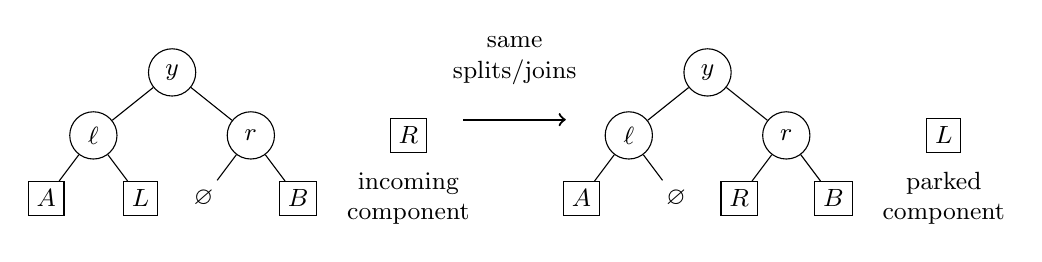
\begin{tikzpicture}[x=1cm,y=1cm,
  key/.style={circle,draw,inner sep=2pt,minimum size=6mm},
  tail/.style={rectangle,draw,inner sep=3pt},
  every node/.style={font=\small}]
\node[key] (y) at (1.8,0) {$y$};
\node[key] (l) at (.8,-.8) {$\ell$};
\node[key] (r) at (2.8,-.8) {$r$};
\node[tail] (a) at (.2,-1.6) {$A$};
\node[tail] (old) at (1.4,-1.6) {$L$};
\node (nil) at (2.2,-1.6) {$\varnothing$};
\node[tail] (b) at (3.4,-1.6) {$B$};
\draw (y)--(l) (y)--(r) (l)--(a) (l)--(old) (r)--(nil) (r)--(b);
\node[tail] (incoming) at (4.8,-.8) {$R$};
\node[align=center] at (4.8,-1.6) {incoming\\component};
\draw[->,thick] (5.5,-.6)--(6.8,-.6);
\node[align=center] at (6.15,.15) {same\footnotesize\\splits/joins};
\begin{scope}[xshift=6.8cm]
\node[key] (yy) at (1.8,0) {$y$};
\node[key] (ll) at (.8,-.8) {$\ell$};
\node[key] (rr) at (2.8,-.8) {$r$};
\node[tail] (aa) at (.2,-1.6) {$A$};
\node (nn) at (1.4,-1.6) {$\varnothing$};
\node[tail] (new) at (2.2,-1.6) {$R$};
\node[tail] (bb) at (3.4,-1.6) {$B$};
\draw (yy)--(ll) (yy)--(rr) (ll)--(aa) (ll)--(nn) (rr)--(new) (rr)--(bb);
\node[tail] (parked) at (4.8,-.8) {$L$};
\node[align=center] at (4.8,-1.6) {parked\\component};
\end{scope}
\end{tikzpicture}
\caption{One left-to-right switch, with the pivot and guards exposed.
The opaque children keep their internal shapes. Equation~\eqref{eq:ms-word}
implements this exchange with explicit common root checkpoints.}
\label{fig:switch}
\end{figure}

Splitting at $y$ performs its full splay. The guard splits perform
exactly the splays stopped at the corresponding child of $y$; removing
$y$ analytically makes those stopped splays ordinary root splays of
the daughter components. The three raw joins restore the guards and
$y$ in exactly the shape produced by the standard switch. Marking the
old tail and unmarking the incoming tail are precisely the corresponding
changes of component membership. Foreign components in the inorder
gaps remain opaque throughout.

If $\ell$ is absent, the first split's entire left daughter is the
parked tail $L$ and the new left daughter is empty. If $r$ is absent,
the new right daughter is simply $R$. Omit the absent guard's split and
join. Right-to-left switches use the reflected operation word. The
same construction applies to the final switch at the requested key;
missing children merely give empty tails.

Consequently there is one fixed mixed forest word $W_{\MS}(X)$,
determined by the reference tree, preferred directions and original
request sequence, with at most six structural operations per switch.
It is independent of the shapes of the auxiliary splay trees. Every
intermediate component has at most $H$ keys, where $H$ is the maximum
preferred-path length. The actual forest splay execution of this word
has exactly the three possible switch splays and their resulting
auxiliary shapes. The original multi-splay search traversal is charged
to these splays by the standard traversal argument; thus its physical
cost is at most a constant times their cost plus $|X|+S_{\MS}$.

For completeness, this traversal charge is pointwise. In each initial
auxiliary exited by the original search, both neighboring keys of the
exit gap lie on its search path. One is the subsequent switch pivot
and the other is one of its ancestor guards. Bottom-up work in deeper
components changes only the incoming opaque payload, so this auxiliary
has not changed before its switch. If the pivot is the deeper of the
two gap neighbors, its first splay already pays the entire old gap
search. Otherwise the first splay pays the path to the pivot, and the
stopped guard splay pays the surviving path below it to the other
neighbor. The final initial auxiliary contains the requested key.
Ancestor switches attach it as an opaque payload, preserving its
internal root-to-query path until the mandatory final query splay.
That last splay pays the remaining initial search segment. Constant
cost per auxiliary boundary is included in $|X|+S_{\MS}$.


\section{The endpoint-aware lower counter}\label{sec:endpoint}
\subsection{The counter to be bounded}

Let $P$ be the perfect node-oriented reference BST on
$n=2^H-1$ keys, whose node depths are $0,\ldots,H-1$.
The initial preferred direction is right at every node. A query $x$
performs the standard multi-splay switches at the ancestors whose
preferences point away from $x$, followed by the final switch at $x$.
The physical ancestor switches run from bottom to top. The analytical
emission list $E_i$ instead lists their depths in increasing order and
appends $\dep(x)$ for the final switch. Thus $E_i$ is strictly increasing.
Write $S_{\MS}=\sum_i|E_i|$.

For a leaf of $P$, the final operation still performs its splays although
there are no children to mark. Give such a leaf a fictitious direction
bit, toggled by this final operation. This bit has no effect on the
physical algorithm; it only makes the encoding uniform.

Let $B$ be any binary interval hierarchy on the depth labels
$0,\ldots,H$. For an internal interval $I=[a,b]$ split at $c$, and a
primary node $u$ of depth $a$, retain an analytical bit $b_{u,I}$,
initially right. An emission $d\in E_i\cap I$ writes left when $d\le c$
and right otherwise, to the bit owned by the depth-$a$ ancestor of
$x_i$. Process $E_i$ in increasing order. Let $F_{\MS}$ count changes of
these bits. There is no extra completion emission $H$ in $E_i$.

\begin{theorem}\label{end:thm:endpoint}
Assume the dynamic lower-bound theorem in the local Tango-squared
manuscript. Then, for the perfect reference above,
\[
 |X|+S_{\MS}(X)+F_{\MS}(X)=O(\OPT(X)+n).
\]
The comparator may choose its initial BST freely. The constant is
independent of $B$ and $H$.
\end{theorem}

The theorem avoids the invalid shortcut of charging every final primary
switch only a constant number of secondary flips. A single extra
emission can change several secondary bits. The proof instead embeds
the entire endpoint-aware history into a legitimate leaf-query history.

\subsection{The lower bound permits arbitrary interval hierarchies}

The Tango-squared manuscript defines a midpoint hierarchy, but its
dynamic lower-bound proof uses only the following properties of that
hierarchy:
\begin{enumerate}
\item For two distinct depth labels, exactly one split separates them.
This is their least common ancestor in the hierarchy.
\item The two children of an interval $[a,b]$ are $[a,c]$ and
$[c+1,b]$. The macro word of the parent is the first child's word;
the micro words are the second child's words, over its different owners.
\item Every nonroot fragment has exactly one parent, so the turn
potentials telescope to the single-depth leaves.
\end{enumerate}
The subsequence-monotonicity proof and the injection of entry and delayed
witnesses use the first property. The normalized MTR simulation and
return property do not use secondary split positions. The turn identity
and its finite occurrence accounting use interval partitions, and the
final telescoping uses the last two properties. No comparison between
the lengths of the two children occurs in these arguments.
Consequently the same proof gives, for any binary interval hierarchy,
\begin{equation}\label{end:eq:lower}
 |Z|+P(Z)+D_B(Z)=O(\OPT(Z)).
\end{equation}
Balancing is relevant to the upper-bound implementation, but not to this
lower-bound extension.

\subsection{A perfect leaf reference with two copies of each key}

Build a full binary primary reference $T$ of height $2H$. An original
node $q$ at depth $d$ corresponds to a pivot $v(q)$ at depth $2d$.
Its two children are connector nodes. Their ordered children are
\[
 \bigl(\text{recursive left subtree of }q,\ q^-\bigr),
 \qquad
 \bigl(q^+,\ \text{recursive right subtree of }q\bigr).
\]
Recursion enters the original children at depth $2d+2$. A copy $q^-$
or $q^+$ denotes one active leaf in the indicated region: if this
region begins above depth $2H$, take its all-right descendant leaf.
Other leaves in that region are inactive. An empty original child
also gives an inactive region. The $2n$ active copies have order
\[
 q_1^-<q_1^+<q_2^-<q_2^+<\cdots<q_n^-<q_n^+.
\]
The two copies of one key are adjacent in the active alphabet, though
there can be inactive leaves between them in the full alphabet.

Call the pivots and the two connectors per original node the
\emph{core}. There are $3n$ core nodes. At depth $a$ the number of core
nodes is at most
\begin{equation}\label{end:eq:core-level}
 2^{\lfloor a/2\rfloor+1}.
\end{equation}
All primary bits of $T$, including the padding, initially point right.

Encode a query to $q$ by the copy on the side opposite to $q$'s current
multi-splay preferred direction. Equivalently, query $q^-$ if the final
switch makes $q$ prefer left, and query $q^+$ if it makes $q$ prefer
right. This defines a leaf-query sequence $Z$ of length $|X|$.

\begin{lemma}\label{end:lem:core}
Immediately before and after every query, the preferred direction of
$v(q)$ equals the multi-splay direction at $q$. During a query the
changes at even-depth core pivots are precisely the multi-splay ancestor
switches and its final switch. Their depths are $2E_i$.
\end{lemma}
\begin{proof}
At a proper ancestor $q$ of the requested original key, either active
copy lies in the same side as that original key. Thus both processes
make exactly the same ancestor preference changes. At the requested
key itself, the chosen copy is on the opposite side of its pivot and
forces exactly its final toggle. No other original pivot is on the
copy's reference path. The initially equal directions therefore remain
equal by induction. Leaf fictitious bits obey the same induction.
\end{proof}

All other noncompletion emissions in $Z$ are at connector nodes.
Padding paths are all-right paths and are only queried at their
all-right active leaf, so no padding preference ever changes.

\subsection{The copies are cheap for every competitor}

\begin{lemma}\label{end:lem:competitor}
For the actual encoded sequence $Z$ on the complete leaf alphabet,
\[
 \OPT(Z)=O(\OPT(X)).
\]
\end{lemma}
\begin{proof}
Replace every node $q$ of an arbitrary competing BST for $X$ by a
two-node gadget: $q^-$ has right child $q^+$, the original left subtree
hangs from $q^-$'s left pointer, and the original right subtree hangs
from $q^+$'s right pointer. A search visits at most two gadget nodes per
original node, and can serve either requested copy.

An original rotation changes only the two adjacent original nodes and
their three hanging subtrees. Its expanded before and after shapes have
at most four gadget nodes and the same ordered hanging subtrees. They
are interconvertible by a constant number of pointer moves and rotations.
The choice of copy may depend on the multi-splay history; the simulation
serves either choice and imposes no restriction on that dependence.

Finally attach the inactive full-alphabet keys as opaque subtrees in
the inorder gaps of the active skeleton. Searches for active copies do
not enter these gap subtrees, and active rotations preserve them. A
comparator may choose this initial full-alphabet tree. Its cost is a
constant multiple of the original execution, without a charge
proportional to the much larger complete reference universe.
\end{proof}

\subsection{Embedding the secondary ledger and its initialization}

Make a hierarchy $B'$ on $0,\ldots,2H$ by replacing each leaf $d<H$
of $B$ by the two leaves $2d,2d+1$, and replacing leaf $H$ by the
single leaf $2H$. An original internal interval $I=[a,b]$ maps to
\[
 J(I)=
 \begin{cases}
 [2a,2b+1],&b<H,\\
 [2a,2H],&b=H.
 \end{cases}
\]
Its split is at $2c+1$. At the corresponding core owner $v(u)$,
an even emission $2d$ therefore writes exactly the same direction as
the original depth $d$ to $b_{u,I}$.

\begin{lemma}\label{end:lem:subsequence}
With all-right initialization, $F_{\MS}(X)\le F_{B'}(Z)$.
\end{lemma}
\begin{proof}
Fix one original owner and interval. In the corresponding $B'$ row,
retain only the even core-pivot emissions. By Lemma~\ref{end:lem:core},
the retained writes, with their chronological order, are precisely the
writes of the original ledger. Removing letters cannot increase the
number of changes in a binary word with a fixed initial letter. Sum
over the injectively corresponding coarse rows of $B'$.
\end{proof}

The nominal complete universe has $2^{2H}$ leaves, so blindly applying
an $O(2^{2H})$ initialization allowance would be useless. The following
support calculation retains the original $O(n)$ allowance.

\begin{lemma}\label{end:lem:initial}
For the encoded history,
\[
 F_{B'}(Z)\le 2D_{B'}(Z)+2P(Z)+18n.
\]
\end{lemma}
\begin{proof}
The initialized-flip conversion in the Tango-squared manuscript gives
the more precise intermediate estimate
\begin{equation}\label{end:eq:precise}
 F_{B'}(Z)\le 2D_{B'}(Z)+3Q_L+2(P(Z)+I_0),
\end{equation}
where $I_0$ counts initial primary changes beyond first-access-free
alternations, and $Q_L$ may be restricted to fragments that ever
receive a left write. Indeed a row receiving only right writes has no
flips and needs no initial-head allowance. Terminal fragments are
already bounded by twice their resets.

Only core primary nodes change, hence $I_0\le3n$. If a fragment
receives a left write, the responsible emission is not the completion
$2H$. It is consequently at a core node. Its owner, at the interval's
left endpoint $a$, is an ancestor of that core node and is itself core.
For an interval split at $c$, $a\le c$, and
\eqref{end:eq:core-level} bounds the number of such owners by
$2^{\lfloor c/2\rfloor+1}$. Distinct internal intervals of a binary
interval hierarchy have distinct split positions. Therefore
\[
 Q_L\le\sum_{c=0}^{2H-1}2^{\lfloor c/2\rfloor+1}
 =4(2^H-1)=4n.
\]
Substituting these estimates in \eqref{end:eq:precise} gives the claim.
\end{proof}

\begin{proof}[Proof of Theorem~\ref{end:thm:endpoint}]
The even core flips are included in all initialized primary flips, so
$S_{\MS}\le P(Z)+3n$. Lemmas~\ref{end:lem:subsequence} and
\ref{end:lem:initial} give
\[
 |X|+S_{\MS}+F_{\MS}
 \le |Z|+2D_{B'}(Z)+3P(Z)+21n
 \le3\bigl(|Z|+D_{B'}(Z)+P(Z)\bigr)+21n.
\]
Apply \eqref{end:eq:lower} and Lemma~\ref{end:lem:competitor}.
\end{proof}

\subsection{Actual order, general size, and initialization}

\begin{lemma}[The actual switch order]\label{end:lem:order}
Let $F_{\MS}^{\mathrm{actual}}$ be the same analytical ledger, now fed
the standard multi-splay order. If
$E_i=(d_1<\cdots<d_k)$, that order is
$(d_{k-1},\ldots,d_1,d_k)$. Then
\[
 \bigl|F_{\MS}^{\mathrm{actual}}-F_{\MS}\bigr|
 \le 2\sum_i\max(|E_i|-2,0)\le2S_{\MS}.
\]
Consequently Theorem~\ref{end:thm:endpoint} also holds with
$F_{\MS}^{\mathrm{actual}}$ in place of $F_{\MS}$.
\end{lemma}
\begin{proof}
Fix one query and restrict its distinct emitted depths to a secondary
interval. A homogeneous left/right block is unchanged. A mixed block
has the form $L^pR^q$ in increasing order. If the interval does not
contain $d_k$, the new block is $R^qL^p$: its internal variation is
unchanged, and each of its two boundary contributions changes by at
most one. If the interval contains $d_k$ and $q=1$, the new block is
still $L^pR$. If it contains $d_k$ and $q\ge2$, the new block is
$R^{q-1}L^pR$: its internal variation increases by one, its last letter
is unchanged, and its entry contribution changes by at most one.
Thus replacing any changed mixed block changes the complete row's
flip count by at most two, including the initialized letter and the
following block if present.

There are exactly $k-1$ secondary intervals meeting both sides of the
emitted set: these are the branching vertices of its induced binary
trie. For $k\ge2$, the parent of the maximum emitted leaf in the
compressed induced trie has only that maximum in its right part.
Its block has $q=1$ and is unchanged. Hence at most $k-2$ mixed blocks
can change. For this query each interval has exactly one owner row;
there is no extra multiplicity from owners. Replace the query blocks
successively in the complete owner-row words and apply the triangle
inequality. This argument does not require a common maximum depth
across queries.
\end{proof}

This order comparison permits the variable final depth of an internal-node query.

\begin{corollary}[Height-optimal references]
Theorem~\ref{end:thm:endpoint}, including Lemma~\ref{end:lem:order}, holds for a
node reference on any $n$ keys whose height in vertices is
$H=\lceil\log_2(n+1)\rceil$.
\end{corollary}
\begin{proof}
The copy construction permits absent original subtrees: the
corresponding portions of the complete embedded reference contain only
inactive leaves. There are still at most $3n$ core vertices. The same
level-count estimate gives
$Q_L\le4(2^H-1)<8n+4$, so the initialization allowance remains $O(n)$.
All correspondence, comparator, and order arguments are unchanged.
\end{proof}

\begin{corollary}[Arbitrary initial primary preferences]
The same bounds hold from any valid initial multi-splay preferred-path
partition, with the same all-right initialization of the analytical
secondary ledger.
\end{corollary}
\begin{proof}
Initialize each embedded pivot $v(q)$ to the supplied initial primary
direction at $q$. Keep the connectors and padding initialized right.
The exact pivot correspondence then holds from the start. The
initialized-primary-flip conversion allows an arbitrary initial
direction, with at most one discrepancy per visited core vertex;
thus $I_0\le3n$ still. Padding vertices remain unchanged. All secondary
rows retain their original right initialization, so the subsequence,
row-support, and order proofs apply verbatim.
\end{proof}

For an arbitrary balanced node reference of maximum depth $H-1$, the
same copy embedding and comparator proof still work. The elementary
initialization estimate is then $Q_L=O(n\operatorname{height}(B'))$,
which is $O(n\log H)$ for a balanced depth hierarchy. The present proof
claims the sharper $O(n)$ allowance for a perfect or height-optimal
reference, including the usual recursively median-split reference.
It does not
silently identify $2^H$ with $n$ for a general balanced reference.


\section{A compatible Tango-squared comparator}\label{sec:comparator}

First let $P$ be perfect, with $n=2^H-1$ keys. View it as a routing
tree on its $n+1$ external gaps. Its internal routing separators are
exactly the original stored keys; this viewpoint adds no physical key.
For a primary path starting at depth $a$, use the depth-exit alphabet
$[a,H]$. Its virtual routing labels are $a,\ldots,H-1$. The unfolding
of \cite{Tango2} uses precisely the original nodes on that path.
Other primary paths are separate components.

The forest word supplies the selected component and the switch pivot.
The comparator therefore processes precisely the actual bottom-up
ancestor switches and then the final switch. At a switch of depth
$d$ it makes a local depth request to $d$; there is no additional
$H$ completion. A final split at the requested node serves that key.
For a real reference leaf, toggling a fictitious null-child direction
only exchanges two different external-gap atoms; the physical tails
are both empty. The ordinary splays and their forest checkpoints remain.

Let $B$ be the fixed balanced interval hierarchy on $0,\ldots,H$.
Write $K_B=1+\operatorname{height}(B)=O(1+\log(H+2))$.
All its balanced path auxiliaries have size at most $K_B$, and their
search, split, and concatenate operations cost $O(\log K_B)=O(\lambda)$.
For brevity in this section $S=S_{\MS}$ and
$F_{\rm act}=F_{\MS}^{\rm actual}$ are the counters from
Section~\ref{sec:endpoint}.

As in \cite{Tango2}, the virtual topology, marks, and genuine bits of
a path occupy $O(H)$ bits stored in its physical root header. Every
use of that header follows a paid visit to the root. Computation on
this already read information is free in the stated model.

\subsection{Local suffix accesses and the histories they really write}

The representation of a path starting at $a$ consists of genuine
canonical intervals $I=[s,t]$ with $s\ge a$, together with a structural
boundary spine $\beta_a$. Set $\beta_0=\varnothing$. For $a>0$,
the spine consists of surviving ancestors of leaf $a-1$ with split
$c\ge a$. It is an all-left chain in the
induced suffix tree, stored in its own balanced auxiliary. Genuine
canonical subtrees hang in its gaps. The seam between its final left
child and the leftmost genuine canonical subtree is administrative:
these are stored in separate auxiliaries even though the boundary
direction is left. Every auxiliary has at most $K_B$ keys.

\begin{lemma}[A local suffix transaction]\label{comp:lem:suffix}
A depth request $a\le d<H$, followed by a primary splice at depth $d$,
can be performed on this suffix representation in
$O((1+f)\lambda)$ pointer and rotation cost, where $f$ counts changes
only at genuine secondary intervals visited by this request. It restores
the same suffix convention at the unchanged starting depth $a$ and
preserves all deeper-owner histories. The old and incoming tails use
the suffix convention at $d+1$.
\end{lemma}

\begin{proof}
First concatenate $\beta_a$ with the root auxiliary of the genuine
subtree at its final left gap, if both exist. This removes the one
administrative seam and gives an ordinary Tango representation of the
induced suffix reference, with all boundary preferences left. This
concatenated auxiliary is a reference path and still has at most $K_B$
keys. One balanced split/join interface costs $O(\lambda)$.

Apply the ordinary Tango access to $d$ in this induced reference. Its
search path leaves the boundary chain through a right edge at most
once. Thus at most one boundary preference changes, in addition to
the $f$ genuine changes. The access costs $O((1+f)\lambda)$ and exposes
the entire induced reference path to leaf $d$ in the root auxiliary.

Apply the exposed splice to this root auxiliary. Its labels greater
than $d$ are exactly the structural boundary of the suffix $[d+1,H]$;
the usual proof by surviving ancestors of leaf $d$ is unchanged by
the restriction to $[a,H]$. Split them off, expose the final two prefix
exit gaps, exchange their roles, and concatenate the incoming
$\beta_{d+1}$. These are constantly many balanced auxiliary operations,
of total cost $O(\lambda)$.

Every crossing genuine interval has owner depth $s\ge a$, contains
$d$, and was just written toward $d$. Its preference therefore agrees
with the new exposed path. Intervals with $s<a$ are structural boundary
nodes, not genuine histories. Intervals with $s>d$ travel with their
respective tails and retain their bits.

Finally restore the unique boundary preference that may have changed
to right. Its split $c$ satisfies $c<d$, so this boundary node survived
in the prefix and its old left continuation was not affected by the
primary splice. One ordinary Tango switch makes it left again. All
boundary preferences are now left and their full chain belongs to the
root auxiliary. Separate its final genuine continuation at the
administrative seam. These two final operations cost $O(\lambda)$,
do not write any genuine bit, and restore the required representation.
If a spine, continuation, or tail is empty the corresponding operation
is omitted.
\end{proof}

\begin{lemma}[Deleted writes, not fictional history updates]\label{comp:lem:deletion}
Across all actual switches, the number $G$ of genuine secondary
changes made by these local suffix accesses satisfies
\[
 G\le F_{\mathrm{act}}.
\]
\end{lemma}

\begin{proof}
Fix one owner row $(I,u)$, where $I=[s,t]$. Delete from its full
$F_{\mathrm{act}}$ write word every event whose selected primary path
starts strictly below $s$. All remaining writes are exactly the
comparator's genuine writes in this row.

Indeed, on a switch at depth $d$ the current preferred path agrees
with the original requested node between its starting depth $a$ and
$d$. Thus whenever $s\ge a$ and $I$ contains $d$, its actual owner is
the fixed primary ancestor at depth $s$ of that request. Whenever
$s<a$, the surviving reference node is structural and supplies no
independent history. A genuine owner bit exists in the component
containing its owner, travels with that owner, and changes only on
these genuine accesses. Lemma~\ref{comp:lem:suffix} shows that a splice
neither resets it nor introduces an unrecorded genuine write.

Both words start from the same initial right bit. Deleting entries
from a binary word cannot increase its variation, by the triangle
inequality between the surviving consecutive bits. Apply this fact
to each fixed owner row and sum. The deletion rule may depend on the
preceding primary states; variation monotonicity needs no independence.
\end{proof}

\subsection{Exposing the original node guards}

The nontrivial transport issue is that a virtual depth label and its
physical unfolding image need not be the same primary separator.
Consequently the presence of routing labels $d-1,d$ in the root
auxiliary alone does not identify the standard multi-splay guards.
The following argument uses actual external gaps instead.

\begin{lemma}[Guard exposure with the same node alphabet]\label{comp:lem:guards}
After the local inner access to depth $d$, an additional $O(\lambda)$
rooted preparation exposes a physical hull containing the switched
key $y$ and both existing nearest-ancestor guards $\ell,r$. This can
be done without changing the common forest domains. It holds even
when one or both primary tails have no internal keys.
\end{lemma}

\begin{proof}
For notation consider a left-to-right switch. In the virtual depth
tree, cut after routing label $d$ as in the exposed-splice lemma,
retaining $d$ with the prefix. Treat the old tail as one opaque
terminal hole. This is a representation of the same current component
$U\cup\{y\}\cup L$: its keys in $L$ remain attached at that hole.
The preparation consists of rotations inside the current component;
it does not execute an early common-forest split.

The last two prefix depth leaves are the off-path exit $E_d$ and the
terminal hole at $d+1$. Routing keys $d$ and, if $d>a$, $d-1$ lie in
the exposed balanced auxiliary. Their two prefix search paths therefore
have $O(\lambda)$ nodes. Rooted-hull unfolding gives physical paths
of that same order. Explicitly walk both paths in the prefix skeleton,
stopping at their gap or at the first root of the opaque attached
subtree. This statement includes null external gaps; it does not
depend on the presence of a header to read.

In the actual prefix alphabet $U\cup\{y\}$, the old left-tail gap
has neighboring keys $\ell,y$, omitting $\ell$ if it does not exist.
The incoming right-tail gap has neighbors $y,r$, with the analogous
omission. Both neighbors of an external BST gap lie on its search path:
the lower neighbor is the last lower bound and the upper neighbor the
last upper bound. Consequently the two explicitly traversed physical
paths contain $y,\ell,r$ whenever present. The same argument applies
when the tails are empty, and reflection handles the opposite switch.

All rotations in the virtual preparation have a rooted physical hull
of size $O(\lambda)$; the two walks add only $O(\lambda)$ nodes.
The rooted touched-hull argument pulls this set back to a rooted hull
in the original component with the same keys and frontier subtrees.
At no point has the old tail ceased to belong to that component.
\end{proof}

\subsection{Inserting the prescribed split and join checkpoints}

\begin{lemma}[Checkpoint insertion]\label{comp:lem:checkpoints}
The suffix transaction of Lemma~\ref{comp:lem:suffix} admits a comparator
execution of precisely the word~\eqref{eq:ms-word}, or its omitted-guard or reflected
version, with cost $O((1+f)\lambda)$. Between consecutive operations
every rotation takes place inside a current common component.
\end{lemma}

\begin{proof}
Carry out the local access and guard preparation inside the selected
component. The incoming tail is selected through its own root handle.
The balanced boundary concatenations may inspect $O(\lambda)$ nodes
of that second component. Keep its inspected set as a second rooted
hull, rather than treating this root selection as an interior jump.
The common interface permits such paid selections and preparation of
another live component between prescribed operations; they do not
change its domain. Equivalently, any preparation entirely inside the
incoming component can be postponed until immediately before the join
that consumes it.

The exposed-splice construction supplies a bounded frontier certificate:
before and after the splice, all untouched physical frontier subtrees
are the same ordered key intervals; the union of touched hull keys
has size $O((1+f)\lambda)$. The old and incoming tail roots are included
when nonempty. This also follows by the usual touched-skeleton tracking:
a move or rotation exposes only its new gap root, and detaching or
attaching a tail exposes its root. Thus each resulting component has
a rooted after-skeleton and the unchanged frontier components.

Use the guard-containing skeleton to prepare the original component
in the form
\begin{equation}\label{comp:eq:before}
y\bigl(\ell(A,L),\ r(\varnothing,B)\bigr).
\end{equation}
Only skeleton keys are rotated. No opaque frontier subtree straddles
one of $y,\ell,r$, since all these keys are in the skeleton. Hence
they can all be preserved while the skeleton is put in \eqref{comp:eq:before}, in time
linear in its size. The subtrees displayed in \eqref{comp:eq:before} include all their
opaque hanging components. The desired internal skeleton shapes
inside $A,L,B$ can be arbitrary at this stage.

Now execute the three specified splits. Their pivots are already
component roots, so each is a legal common root deletion. The old
tail $L$ becomes a separate component exactly at its specified split,
and no earlier. Perform the three raw root joins of~\eqref{eq:ms-word}, with the
prescribed domains and pivots. They give
\begin{equation}\label{comp:eq:after}
y\bigl(\ell(A,\varnothing),\ r(R,B)\bigr)
\end{equation}
and the parked component $L$.

Finally reconfigure the portions of the skeleton in these resulting
components to the valid after-representations prescribed by the
exposed splice and by boundary restoration. Each is a rooted skeleton
with the same ordered frontier intervals; linear-cost BST reconfiguration
therefore applies separately inside each component. No rotation crosses
a component boundary. An absent guard simply removes its split, join,
and displayed skeleton node. If both tails are empty, the same
guard preparation and checkpoints are performed; the argument never
relied on a nonempty tail.

The preparation, six checkpoints, and final reconfigurations cost
$O((1+f)\lambda)$ in total. They end with the required persistent owner
histories, because those histories were specified by the ideal local
suffix transaction and have not been initialized again.
\end{proof}

\begin{theorem}[Common-word comparator]\label{comp:thm:comparator}
The exact multi-splay forest word has a comparator of cost
\begin{equation}\label{comp:eq:count}
C_{\mathrm{forest}}(W_{\MS}(X))
   =O\bigl(n+\lambda(S+F_{\mathrm{act}})\bigr).
\end{equation}
The endpoint count theorem consequently gives
\begin{equation}\label{comp:eq:opt}
C_{\mathrm{forest}}(W_{\MS}(X))
   =O\bigl(\lambda(\OPT(X)+n)\bigr).
\end{equation}
\end{theorem}

\begin{proof}
Initialize every path's balanced suffix representation with the
all-right genuine histories, in total $O(n)$ work. A component with
$k$ keys can be changed to its prescribed initial shape in $O(k)$
rooted rotations and moves. Sum Lemma~\ref{comp:lem:checkpoints} over the
$S$ switches, and use Lemma~\ref{comp:lem:deletion}. This gives \eqref{comp:eq:count} with
no lifetime initialization charge and no persistent splay potential:
the comparator's auxiliaries are balanced.

The endpoint embedding and actual-order lemma of Section~\ref{sec:endpoint} give
$S+F_{\mathrm{act}}=O(\OPT(X)+n)$ for this exact emission stream.
Substitution yields \eqref{comp:eq:opt}.
\end{proof}

\subsection{Padding the reference without adding physical keys}

The comparator construction also applies to the customary minimum-height
balanced reference on an arbitrary number $n$ of keys. Put
$H=\lceil\log_2(n+1)\rceil$. Complete its routing reference to depth
$H$ by adding conceptual dummy routing nodes below each original
external gap. Within each such padded gap region, retain only its
all-right depth-$H$ descendant as an \emph{active} gap representative.
Every other padded leaf is inactive. There are still exactly $n+1$
active external gaps, in their original order.

Give every dummy primary vertex the fixed right preference. It has
at most one active child, whereas every original vertex has two active
children. Suppressing the inactive pieces and unary refinements
therefore yields exactly the original node-storing reference, with
each original separator once and no physical dummy key. Complete the
secondary virtual alphabet to $0,\ldots,H$ as before.

The unfolding proof continues to hold with empty components suppressed:
a depth interval has at most two active interval components, an
abstract routing node has at most two physical images, and the same
rooted-hull and equal-frontier proofs apply. Here an active external
gap is retained as an ordered atom even when it contains no stored
key. Thus the two null child gaps at a real primary leaf remain
different active atoms separated by that leaf's real key. In
particular the two-gap guard argument does not disappear when both
tails are physically empty.

Every emitted depth belongs to a real switched node. Every owner
ancestor at an earlier or equal depth is therefore real as well.
No genuine row whose owner is dummy ever receives a write; all such
bits stay right. A physically empty tail lies entirely in a dummy
region, so all its genuine histories and its structural boundary can
be reconstructed from its starting depth and region. Its auxiliary
shape can be chosen canonically without physical work. This introduces
no potential reset, because the comparator uses balanced auxiliaries
and has no shape potential. A nonempty component stores all its
nonconstant virtual histories in the same $O(H)$-bit header as before.

Consequently the proof of \eqref{comp:eq:count} holds unchanged for arbitrary $n$ and
the exact original forest word. No split or join at a dummy pivot is
inserted. The completed reference has fewer than $2n+1$ internal
vertices, so any linear reference-count initialization allowance also
remains $O(n)$. The endpoint corollary for minimum-height references in
Section~\ref{sec:endpoint} supplies \eqref{comp:eq:opt} for this reference too.


\section{One persistent Splay comparison forest}\label{sec:forest}
\subsection{Existing local normal-form interfaces}

Write $L_K=1+\lceil\log_2(K+1)\rceil$. The repository has two
representation layers with exactly the required root operations.

\paragraph{The heavy-path layer.}
\texttt{OfflineHeavyJoin.lean} proves the root-join interface
\texttt{exists\_join} for a heavy representation;
\texttt{OfflineHeavySplit.lean} proves \texttt{exists\_split\_node}.
For either operation there is an exposed
supported path of cost $c_H$ satisfying
\[
 c_H\le 16L_K^2+3,
 \qquad
 c_H+\Phi_H(\text{after})
 \le\Phi_H(\text{before})+115.
\]
Before and after potentials are summed over the participating children
when the state is a forest. Every represented tree has height at most
$6\lceil\log_2(K+1)\rceil^2$. The potential bound
\texttt{OfflineHeavyPotential.lean} is
\[
 0\le\Phi_H(T)\le64|T|.
\]
The split theorem expressly returns the child representation histories.

\paragraph{The rib layer.}
\texttt{OfflineRibRootOperations.lean} proves a root join and root
split with
\[
 c_R\le64L_K^2,
 \qquad
 c_R+\Phi_R(\text{after})
 \le\Phi_R(\text{before})+448.
\]
A join requests a left representation with orientation \texttt{true}
and a right representation with orientation \texttt{false}.
The same file proves \texttt{exists\_reorient} for either desired
orientation, with
\[
 c_{\mathrm{orient}}\le128L_K^2,
 \qquad
 c_{\mathrm{orient}}+\Phi_R(\text{after})
 \le\Phi_R(\text{before})+896.
\]
This operation preserves the represented source tree. It consists of
two root stack operations, rather than a reconstruction of the component.
\texttt{OfflineRibPotential.lean} gives
$0\le\Phi_R(T)\le256|T|$.

Rib representations have bounded minor ribs, with slack nineteen, and
increase source height by at most a factor
$5\lceil\log_2(K+1)\rceil$.
The supported-path conversion in
\texttt{OfflineRestrictedMacros.lean} and
\texttt{OfflineRibbedTrace.lean} replaces each supported macro by
root or grandchild rotations at constant overhead in its support size.
It preserves a height bound equal to the endpoint height plus the
support size, and a constant minor-rib bound (slack twenty for the
ribbed construction).

The underlying representation, rotation, split and join statements are
parameterized by a \emph{capacity}. It is therefore legitimate to use the
same fixed capacity $K$ throughout an evolving forest. Changing a
component's size does not require changing its representation parameter.
The exported \texttt{exists\_boundedService} and
\texttt{exists\_boundedRotation} corollaries specialize that capacity to
the dense alphabet size. Here their proofs are applied with arbitrary
capacity $K$: the displayed support and potential inequalities come from
the underlying capacity-parameterized interfaces, and their conversion
to shallow traces is unchanged. This lifting is part of the present
hand argument, not an existing forest theorem in Lean.

A live component's possibly nonconsecutive keys can be relabeled by
their inorder positions for these local statements. Splitting or joining
changes this order isomorphism but changes no physical tree shape,
rotation, stack digit, supported frontier, or potential. Transport the
existing representation witnesses through the new order isomorphism;
do not choose fresh representations. Thus alphabet relabeling itself
performs no pointer operations and grants no access to an interior node.

\subsection{The forest normal form}

\begin{theorem}[Common forest normalization]\label{forest:thm:normal}
Every comparator execution of the interface above has a common-domain
comparison forest with total cost
\[
 O(C+N+q),
\]
height $O(L_K^3)$ in every physical intermediate tree, a constant bound
on minor ribs, and all rotations at constant depth within the component
being processed. Immediately before a split and immediately after the
common raw join, the relevant pivot is the root. All surviving child
representation histories are retained across the structural operations.
\end{theorem}

\begin{proof}
First replace each root-starting comparator transaction by shallow
rotations of its touched rooted hull, retaining the same hanging
subtrees. This is the usual constant-cost restricted-rotation conversion,
applied inside the selected component. A split first exposes its
requested pivot as a root; a join is a raw common root insertion followed
by any further comparator work. This gives $O(C+q)$ root services,
shallow rotations, root deletions and root insertions.

Maintain a heavy representation of each component at fixed capacity
$K$. The supported rotation and service interfaces already used in
\texttt{OfflineHeavyBoundedSteps.lean} handle the fixed-domain work.
Use the explicit heavy split and join interfaces for the structural
operations. The raw join $x(A,B)$ has height at most one more than the
maximum child height, so it also satisfies an $O(L_K^2)$ bound.
The supported paths have size $O(L_K^2)$; conversion to shallow rotations
therefore keeps all intermediate heights $O(L_K^2)$.

Sum the heavy potential over all live components. A split replaces one
summand by its two surviving child summands, and a join performs the
reverse accounting operation with a new pivot. The initial potential is
at most $64N$. Each primitive supplies only its stated constant
amortized allowance. Nonnegativity of the final global potential gives
$O(C+q+N)$ total work in this first representation layer. There is no
component-lifetime initialization sum.

Apply the rib representation to the resulting shallow trace, again
retaining its histories at fixed capacity $K$. Before a raw root join,
reorient the two child representations as necessary. There are at most
two such reorientations. Insert the common pivot above the children,
then apply the rib join interface. Its source has bounded minor ribs
because of the chosen child orientations; this is the same exposed-root
geometry used by \texttt{exists\_boundedService} in
\texttt{OfflineRibBoundedSteps.lean}. Its height is one more than the
maximum child height. A root split is handled by exposing the source
root with \texttt{exists\_split\_node}, deleting that root, and retaining
the two returned child representations. Their returned orientations may
be kept until a later join requires a change.

The rib height is $O(L_K)$ times the first layer's $O(L_K^2)$ height;
the $O(L_K^2)$ supported-path allowance is smaller. Supported-path
conversion keeps this $O(L_K^3)$ height and constant minor-rib bound
throughout every macro. Its rotations stay at constant depth.

Finally sum the rib potential over live components. Its initial sum is
at most $256N$. A root join costs at most two reorientation allowances
and one join allowance; a split costs one split allowance. The existing
rotation and service allowances charge the rest of the first-layer
trace. The potentials telescope with the actual child histories.
Thus the second layer costs $O(C+q+N)$ as well.

For synchronization, expose the comparison pivot before the algorithm's
splay for a split, and delete the common root only afterwards. At a
join, perform any orientation changes while the children are still
separate; then both forests receive the same raw root $x$. Subsequent
comparison normalization rotations are ordinary paid comparator changes.
This establishes the stated common-root checkpoints.
\end{proof}

This proof is an application of the local existing interfaces. A Lean
formalization would additionally need a forest trace type, the global
sum of component potentials, and order-isomorphism transport between
component alphabets. These are not supplied by the existing fixed-domain
\texttt{RibbedTrace} datatype.

\subsection{Root joins in the splay accounting state}

\begin{lemma}[Common root join accounting]\label{forest:lem:heap-join}
Suppose the splay and comparison forests join the same two domains
under a new common root $x$. The lazy-interval accounting state of the
splay manuscript can retain all old states and perform only $O(1)$ new
interface and potential events for this operation.
\end{lemma}

\begin{proof}
Immediately before the join, ranks in each child are measured from
the root of its own comparison component. After the common raw join,
increase all old ranks in each child by one and give $x$ rank zero.
All differences between old ranks within a child are unchanged.
Consequently all internal gaps, point gaps, heavy paths and lazy
intervals of that child retain their previous state.

The new minimum $x$ becomes the root heavy path. The previous root
heavy path of each nonempty child becomes one left or right heap child
of $x$. Its minimum comparison rank used to be zero and is now one,
so its new gap is one. Create the two possible growing singleton
intervals at $x$ and their constant-size records. This introduces only
$O(1)$ point-gap contributions and boundary events, and only $O(1)$
new bends. All records internal to the children remain in place.

More explicitly, the old child-root has interface value $f=1$ from
its root point gap zero. Its new singleton gap one has contracted
value $f=2$. Apply one \texttt{ValueIncrease} to this child root,
\texttt{Create} the corresponding growing parent slot at value one,
and \texttt{Insert} the child at value two. The insertion inequality
is $2\ge1+1$, and there are at most two such children. The inverse
root deletion first \texttt{Convert}s these root singletons, returning
the child's value from two to one, and then deletes them. Empty
growing slots of the removed pivot are converted and retired. On
reinsertion its newly created slots again start at value one.
Child intervals, pass counts, and creator histories are retained.

This is the reverse of the common root deletion in
\texttt{app-split-conjecture.tex}, except that insertion is charged its
constant number of new records. Reinserting a formerly deleted pivot
creates those records again and is paid again as one of the $q$
structural operations. It does not recreate the children's records.
One can place every key that will occur into the interface universe
in advance, giving an inactive key the neutral value $f=1$ and
charging the initial excess $\sum(f-1)$. Alternatively, its size is
at most the $N$ initially active keys plus the $q$ insertion events.
Either convention charges future pivot lifetimes by $O(N+q)$ and
does not reset a live child's potential.
Subsequent comparison normalization rotations are handled by the
ordinary paid-rotation part of the original proof.
\end{proof}

\begin{theorem}[Common-forest splay comparison]\label{forest:thm:splay}
Assuming the core lazy-interval and pairing-accounting argument of the
current splay manuscript, its comparison extends to the interface above
with
\[
 \cost_{\mathrm{splay\ forest}}
 =O\!\left((C+N+q)\,
   (1+\log\log(K+4))
   (1+\log\log\log(K+16))^2\right).
\]
\end{theorem}

\begin{proof}
Use Theorem~\ref{forest:thm:normal} as the comparison forest. Its ranks lie in
$O(L_K^3)$, so the maximum contracted rank gap is $O(1+\log\log(K+4))$.
The two logarithmic losses from the existing lazy-interval accounting
are $O(1+\log\log\log(K+16))$ each.

The original forest has $O(N)$ initial records. Ordinary splays and
paid comparison rotations create the already established constant
number of records per event. Common root deletion uses the unchanged
split argument; Lemma~\ref{forest:lem:heap-join} handles common root insertion.
Thus all record and boundary budgets are $O(C+N+q)$, and the original
global pairing and bend estimates sum over the live components.
No potential is restarted at a split or join.

Here is the global accounting explicitly. Set $B_0=N+C+q$ and let
$G\ge2$ bound the contracted gaps. Let $\ell$ count created lazy
intervals, $p$ paid interface operations, $u$ unimportant boundary
pairings, $g$ good internal pairings, and $A$ all internal pairings.
The retained-history construction and the local splay estimates give
\[
 \ell=O(B_0),\qquad
 p\le u+O(B_0\log G),\qquad
 g\le uG+O(B_0G\log G).
\]
Root joins add only $O(q)$ inserts and value increases. Thus the
interface totals satisfy
\[
 \#\texttt{Insert}=O(p+N+q),\qquad
 \#\texttt{ValueChange}=O\bigl(g+(p+N+q)G\bigr).
\]
The original pairing inequality consequently remains
$A\le\alpha(pG\log G+O(B_0G\log^2G))+O(1)$ for its fixed constant
$\alpha$. The same definition of unimportance supplies
$\alpha uG\log G\le A/2$. Absorbing this term gives
$A=O(B_0G\log^2G)$. Important boundary pairings contribute
$O(B_0\log G)$, and unimportant ones are absorbed as before. Joins
and splits add $O(q)$ bends, so the zig-zag count has the same bound.
Taking $G=O(1+\log\log(K+4))$ gives the displayed theorem.
\end{proof}


\section{Composition and the competitive factor}

\begin{proof}[Proof of Theorem~\ref{thm:main}]
The endpoint theorem and its actual-order corollary give
\[
 |X|+S+F_{\rm act}=O(\OPT(X)+n).
\]
The compatible comparator of Section~\ref{sec:comparator} therefore
costs $C_{\rm forest}=O(\lambda(\OPT(X)+n))$. Apply
Theorem~\ref{forest:thm:splay} to the exact word
$W_{\MS}(X)$. It has $n$ initially active keys, at most $6S$
structural operations, and component capacity $K=H$. Its splay
execution is precisely the auxiliary splay execution of multi-splay.
The traversal charge of Section~\ref{sec:word} includes the remaining
physical search work. Consequently
\[
 \cost_{\MS}(X)
 =O\bigl((C_{\rm forest}+n+S)g(H)\bigr)
 =O\bigl((\OPT(X)+n)\lambda g(H)\bigr).
\]
Substituting $H=\lceil\log_2(n+1)\rceil$ gives~\eqref{eq:main}.
\end{proof}

\paragraph{What is needed for the stronger ratio.}
The present derivation pays $\lambda$ for the compatible Tango-squared
comparator and $g(H)$ for the splay forest; neither loss disappears
under composition. An $O(\OPT+n)$ comparator for the same complete
word would remove the first loss and give
$O((1+\lgit{3}n)(1+\lgit{4}n)^2)$ instead. The exact
$O(\lgit{3}n)$ target requires a further improvement. This paper does
not claim either stronger statement.

\paragraph{Why the whole forest matters.}
The proof does not restart a fixed-universe Splay theorem at every
new preferred path. Such restarting would charge the lengths of newly
formed paths repeatedly, even on repeated root requests whose actual
cost is constant. The preserved child representations and preserved
lazy histories are the mechanisms that remove this spurious charge.
Likewise, the comparator theorem concerns the complete guard split/join
word, not just the original query sequence or a query-only inner Tango
execution.

\section{Proof status and dependency record}

The endpoint embedding, switch-order estimate, mixed-forest composition,
suffix transaction, and exact checkpoint insertion were independently
hand-audited. The Splay repository already contains checked local heavy
and rib interfaces used in Section~\ref{sec:forest}. The Tango-squared
repository contains a checked lower endpoint for its stated midpoint
hierarchy and a hand physical upper construction. The arbitrary
secondary hierarchy extension in Section~\ref{sec:endpoint}, the forest
trace composition, and the composed theorem here have not been added
as Lean theorems. The mathematical dependencies are the stated core
proofs of \cite{Splay,Tango2}, rather than the existence of a compiled
PDF or the outcome of finite tests.

The source of this paper is self-contained apart from those two core
proof dependencies. The supporting research notes contain finite checks
of the endpoint identities, suffix-state transport, and fixed-path
unfolding; these checks support their specified identities only and
are not used as substitutes for any theorem above.

\begin{thebibliography}{9}
\bibitem{Splay}
P.~Chmel, B.~Haeupler, R.~Hlad\'ik, M.~Kouck\'y, A.~Roeyskoe,
V.~Rozho\v{n}, O.~Sladk\'y, and R.~E.~Tarjan.
\emph{Splay trees are almost dynamically optimal}.
2026. \url{https://arxiv.org/abs/2607.18498}.
The current local manuscript, especially its normal-form and split
appendices, and its checked accounting interfaces are used here.

\bibitem{Tango2}
\emph{Tango Squared: An $O(\log\log\log n)$-Competitive Binary
Search Tree}. Current local research manuscript, October 2026.
Source: \texttt{tango\_squared/research/tango-squared.tex}.
The dynamic lower bound, initialized flip conversion, no-copy unfolding,
rooted-hull transfer, suffix invariant, and exposed splice are the
imported results.

\bibitem{MST}
C.~C.~Wang, J.~Derryberry, and D.~D.~Sleator.
\emph{$O(\log\log n)$-Competitive Dynamic Binary Search Trees}.
SODA 2006.
\url{https://www.cs.cmu.edu/~jonderry/multi-splay.pdf}.

\bibitem{Wang}
C.~C.~Wang. \emph{Multi-Splay Trees}. PhD thesis,
Carnegie Mellon University, 2006. CMU-CS-06-140.
\url{https://www.csd.cmu.edu/sites/default/files/phd-thesis/CMU-CS-06-140.pdf}.
Sections 3.2--3.4 specify the switch and traversal conventions.
\end{thebibliography}
\end{document}
